\chapter{Antecedentes y motivaci\'on.}

% \hspace*{0.4 cm} La curva de redimientos es una herramienta ampliamente utilizada por las autoridades de los bancos centrales en sus decisiones de pol\'itica monetaria, as\'i como tambi\'en por los agentes privados en la planificaci\'on de sus inversiones en instrumentos financieros [1]. La misma tiene una importancia capital
% para el mundo acad\'emico y pr\'actico desde el punto de vista econ\'omico y financiero, al reflejar el precio intertemporal del dinero.

\section{Rendimiento.}

\hspace*{0.4 cm} El rendimiento es un t\'ermino utilizado en finanzas, bancos, t\'itulos y valores financieros, es el producto o utilidad que se obtiene de algo  de alguna inversi\'on. Es frecuente en \'epocas de inflaci\'on, que los intereses que otorguen otros instrumentos de inversi\'on, sean superiores a los que otorgan los bonos y obligaciones que llevan varios a\~nos de haberse emitido, lo cual resta inter\'es a la adquisici\'on de dichos bonos a menos que se les descuente en su precio la cantidad necesaria para hacerlos competitivos.

\hspace*{0.4 cm}Es as\'i como empiezan a operar los bonos y las obligaciones, ``con descuento", o ``abajo de su valor nominal". Quien compra un bono u obligaci\'on ``abajo de su valor nominal", espera recibir un inter\'es atractivo y, adicionalmente, una ganancia de capital en el momento en que venda el bono.

\hspace*{0.4 cm}El bono u obligaci\'on ir\'a subiendo de precio, hasta que llega a coincidir con el valor nominal, el d\'ia de su vencimiento. Es frecuente que los bonos y obligaciones no lleguen al vencimiento al $100\%$ el mismo d\'ia, sino que tengan amortizaciones previas (predefinidas) por sorteo o por serie. En estos casos, hay que emplear f\'ormulas especiales para llegar al rendimiento y vencimiento incluyendo las amortizaciones.

\subsection{Tipos de rendimiento.\\}

\hspace*{0.4 cm} En base al precio vigente, un bono muestra tres diferentes tipos de vencimiento,

\begin{itemize}
  \item El rendimiento del cup\'on es la tasa de inter\'es que paga el bono por su valor nominal. Un bono de $US\$10.000$ con un cup\'on del 6 por ciento de inter\'es paga $US\$300$ de inter\'es cada 6 meses.
  \item El rendimiento actual es la tasa del cup\'on dividida por el precio del bono. Si el bono con un valor nominal de $US\$10.000$ y un 6 por ciento de tasa de cup\'on puede ser comprado por $US\$9.600$, su rendimiento actual es de 6,25 por ciento. 
  \item El rendimiento al vencimiento es la tasa interna de retorno del bono en funci\'on del tiempo que falta para el vencimiento del bono.
\end{itemize}


\subsection{Bonos bajo y sobre la par.\\}

\hspace*{0.4 cm} Los bonos suelen venderse bajo la par o sobre la par. Un bono con una alta tasa de cup\'on cuando las tasas de mercado son bajas se vender\'a sobre la par. Los bonos se vender\'an bajo la par si la tasa del cup\'on es m\'as baja que la de mercado para bonos similares. A los inversores novatos les gusta la idea de comprar bonos bajo la par, creyendo que est\'an comprando barato. En verdad, un bono cotizado sobre la par puede ser una mejor inversi\'on. El inversor recibir\'a pagos de inter\'es m\'as altos que podr\'a reinvertir.

\hspace*{0.4 cm} El c\'alculo del rendimiento al vencimiento amortiza el valor de la prima o el descuento (bonos sobre y bajo la par) en el precio del bono a lo largo de la vida que le queda al bono. Por ejemplo, si el bono que paga 6 por ciento de tasa de cup\'on mencionado anteriormente vence en 10 a\~nos, y tiene un precio de $US\$9.600$, el rendimiento al vencimiento es 6,558 por ciento. Si dos bonos, uno sobre la par y otro bajo la par, tienen el mismo rendimiento al vencimiento, cualquiera de ellos representa el mismo nivel de retorno para el inversor. El rendimiento al vencimiento es lo que el inversor recibir\'a si el bono es comprado al precio vigente en el mercado y sostenido hasta su vencimiento.

\hspace*{0.4 cm} Algunas reglas sencillas ayudan a los inversores a entender la relaci\'on de el rendimiento al vencimiento de un bono y otras medidas de rendimiento. Para un bono sobre la par, el rendimiento al vencimiento es m\'as bajo que el rendimiento actual, que a su vez es m\'as bajo que la tasa de cup\'on. Con un bono bajo la par, el rendimiento al vencimiento es la tasa m\'as alta, seguida por el rendimiento actual, siendo la tasa de cup\'on el indicador m\'as bajo.


\section{Curva de rendimientos.}

\hspace*{0.4 cm} La curva de rendimientos es una representaci\'on grafica que muestra la relaci\'on que existe entre los rendimientos de una clase particular de t\'itulos valores y el tiempo que falta para su vencimiento, lo cual es conocido como la estructura temporal de la tasa de inter\'es (ETTI) para instrumentos con riesgo similar pero con diferentes plazos de maduraci\'on. La ETTI es un indicador de la evoluci\'on futura de los tipos de inter\'es y de inflaci\'on, adem\'as, la mayor\'ia de los activos financieros se valoran mediante este indicador, por lo cual tambi\'en se considera b\'asico en el dise\~no de estrategias de gesti\'on de riesgos y en la toma de decisiones de inversi\'on y financiaci\'on \cite{FR}. Existen cuatro formas que puede adoptar una curva de rendimientos:

\begin{itemize}
  \item \textbf{Curva ascendente}: generalmente, la curva de rendimientos tiene esta      forma, lo que indica que los inversionistas requieren mayores rendimientos     para vencimientos de m\'as largo plazo, es decir, que los rendimientos         var\'ian directamente con los plazos. 
  \item \textbf{Curva descendente}: indica que los rendimientos disminuyen a medida que   aumentan los plazos.
  % \item Curva horizontal: indica que independientemente del plazo de vencimient   o, los rendimientos son los mismos; para per\'iodos muy largos, todas las      curvas de rendimientos tienden a aplanarse.
\end{itemize}

\begin{itemize}
   \item \textbf{Curva horizontal}: indica que independientemente del plazo de vencimiento, los rendimientos son los mismos; para per\'iodos muy largos, todas las      curvas de rendimientos tienden a aplanarse.
\end{itemize}


\begin{itemize}
  \item \textbf{Curva creciente y decreciente}: es el reflejo de una situaci\'on en la    que los rendimientos de corto y largo plazo son los mismos y los rendimientos  de mediano plazo son los que var\'ian.
\end{itemize}

\begin{figure}[h]
  \scalebox{0.80}{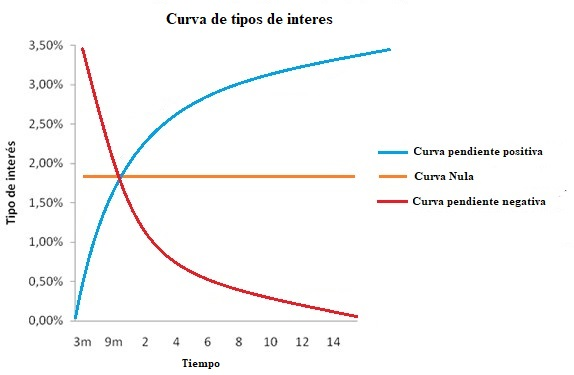
\includegraphics{images/tipo_curvas.jpg}}
\caption{Tipos de curva de rendimiento.}
\label{tipos_c}
\end{figure}

\hspace*{0.4 cm} Es de esperar que una pendiente negativa de la curva de rendimientos (Ver Figura \ref{tipos_c}) o curva invertida (tasas de largo plazo menores a las de corto plazo) indique expectativas de una recesi\'on futura y, por lo tanto, menores tasas de inter\'es futuras; esto se puede explicar ya que los rendimientos esperados contienen informaci\'on sobre los planes de consumo de los agentes. 

\hspace*{0.4 cm} Entre las teor\'ias que explican la pendiente de la curva de rendimientos, se encuentran:

\begin{itemize}
  \item \textbf{La teor\'ia de la preferencia por la liquidez}: consiste en que los inversionistas prefieren manejar t\'itulos a corto plazo, pues \'estos tienen una sensibilidad menor a los cambios en las tasas de inter\'es y ofrecen una mayor flexibilidad en las inversiones si se compara con los t\'itulos de largo plazo. Adem\'as, los prestatarios prefieren deuda a largo plazo, pues la de corto plazo los expone al riesgo de hacer una refinanciaci\'on de la deuda en condiciones adversas. Ambas situaciones, generan entonces, tasas de corto plazo relativamente bajas. En su conjunto, estos dos grupos de preferencias implican que en condiciones normales existe una Prima de Riesgo por Vencimiento (PRV) que aumenta en funci\'on de los a\~nos de vencimiento, haciendo que la curva de rendimientos posea una pendiente ascendente \cite{DO}.
  \item \textbf{La teor\'ia de la segmentaci\'on del mercado}: considera el mercado de renta fija como una serie de distintos mercados, los inversionistas y los emisores est\'an restringidos por el sector espec\'ifico de maduraci\'on. De acuerdo con esta teor\'ia, la curva de rendimientos refleja una serie de condiciones de oferta y demanda que crean una secuencia de precios de equilibrio de mercado (tasas de inter\'es) de los fondos \cite{DO}.
  \item \textbf{La teor\'ia del H\'abitat Preferido}: plantea que los inversionistas intentar\'an liquidar sus inversiones en el menor plazo posible mientras que los prestamistas querr\'an tomar un plazo m\'as largo; por lo tanto, dado que no se encuentran oferta y demanda de fondos para un mismo plazo, algunos inversionistas o prestatarios se ver\'an motivados a cambiar el plazo de la inversi\'on o el financiamiento pero, para lograrlo, deben ser compensados con un premio por el riesgo cuyo tamano reflejar\'a la extesi\'on de la aversi\'on al riesgo.
  \item \textbf{La Hip\'otesis de las Expectativas (HE)}: plantea que las tasas de inter\'es de largo plazo deben reflejar por completo la informaci\'on revelada por las futuras tasas de inter\'es de corto plazo esperadas \cite{YS}, o sea que los tipos de largo plazo no son m\'as que una suma ponderada de los tipos de corto plazo esperados \cite{FR}. As\'i, se puede afirmar entonces que la HE es una teor\'ia que plantea que las tasas de inter\'es exclusivamente representan las tasas previstas en el futuro.
\end{itemize}



\section{Deuda P\'ublica Nacional.}

\hspace*{0.4 cm} Uno de los principales objetivos que se persigue mediante el uso de la curva de rendimientos es el de estimar los precios de los t\'itulos de la deuda p\'ublica nacional que posee una instituci\'on financiera en su portafolio de inversiones en un per\'iodo determinado. 


% \hspace*{0.4 cm} Por una parte se tiene que deuda es la obligaci\'on que un sujeto tiene de reintegrar, satisfacer o pagar, especialmente dinero. P\'ublico, por otra parte, es un adjetivo que refiere a aquello perteneciente a toda la sociedad o que es com\'un del pueblo.

\hspace*{0.4 cm} La noci\'on de deuda p\'ublica hace menci\'on al conjunto de deudas que mantiene el Estado frente a otro pa\'is o particulares. Se trata de un mecanismo para obtener recursos financieros a trav\'es de la emisi\'on de t\'itulos de valores.

\hspace*{0.4 cm} El Estado, por lo tanto, contrae deuda p\'ublica para solucionar problemas de liquidez (cuando el dinero en caja no resulta suficiente para afrontar los pagos inmediatos) o para financiar proyectos a medio o largo plazo. La deuda p\'ublica puede ser contra\'ida por la administraci\'on municipal, provincial o nacional. Al emitir t\'itulos de valores y colocarlos en los mercados nacionales o extranjeros, el Estado promete un futuro pago con intereses seg\'un los plazos estipulados por el bono.

\hspace*{0.4 cm} La emisi\'on de deuda p\'ublica, al igual que la creaci\'on de dinero y los impuestos, son medios que tiene el Estado para financiar sus actividades. La deuda p\'ublica, de todos modos, tambi\'en puede utilizarse como un instrumento de la pol\'itica econ\'omica, de acuerdo a la estrategia escogida por las autoridades. Tendr\'iamos que hablar, por un lado, de tres tipos diferentes de deuda p\'ublica, aunque es cierto que hay diversas clasificaciones. Una clasificaci\'on de la deuda, es la siguiente,

\begin{itemize}
  \item \textbf{A corto plazo}: Dentro de esta categor\'ia se encuentran las Letras del Tesoro y se identifica por el hecho de que tiene un plazo de vencimiento que no supera el a\~no.
  \item \textbf{A medio plazo}: Los bonos del Estado son los m\'aximos exponentes de esta clase de deuda p\'ublica que se suele utilizar para hacer frente a lo que ser\'an los gastos ordinarios.
  \item \textbf{A largo plazo}: Como su propio nombre indica, este tipo de deuda tiene una duraci\'on muy larga, que se fijar\'a convenientemente, y que puede incluso llegar a ser perpetua. 
\end{itemize}


\hspace*{0.4 cm} Otra posible clasificasi\'on de la deuda p\'ublica se presenta a continuaci\'on. La deuda p\'ublica real es aquella compuesta por los t\'itulos que pueden ser adquiridos por los particulares, los bancos privados y el sector exterior. La deuda p\'ublica ficticia, en cambio, es la emisi\'on destinada al Banco Central del pa\'is, que es un organismo de la misma administraci\'on p\'ublica.





% \hspace*{0.4 cm} Con el fin de calcular o estimar los precios de los t\'itulos \'o instrumentos de deuda p\'ublica nacional que existen en el mercado venezolano es importante conocer las caracter\'isticas de los mismos, entre ellos tenemos los siguientes,
% 
% \vspace{0.4cm}
% 
% \begin{itemize}
%   \item T\'itulos de inter\'es fijo (TIF): son instrumentos que se caracterizan por tener una renta fija, y se emiten en moneda nacional.
%   \item T\'itulos de inter\'es variable (VEBONO): se caracterizan por poseer una renta variable, e igual que los TIF se emiten en Bol\'ivares.
%   \item Bonos PDVSA : son instrumentos emitidos en d\'olares.
% \end{itemize}
% 
% \vspace{0.5cm}
% 
% \noindent cabe destacar que en el presente trabajo s\'olo  se considerar\'an aquellos instrumentos emitidos en Bol\'ivares.
% 
% \vspace{0.5cm}
% 
% \hspace*{0.4 cm}Asociado a cada t\'itulo hay un monto de dinero que se invierte, el cual es entregado al ente emisor por el t\'itulo en s\'i, existe tambi\'en una fecha de emisi\'on, y una fecha de vencimiento, d\'ia en el cual el ente emisor retorna el monto invertido inicialmente. Es importante destacar que estos t\'itulos pagan un inter\'es al portador cada tres meses, y esta representa la ganancia que tiene el inversionista.
% 
% \vspace{0.5cm}
% 
% \hspace*{0.4 cm} Con el fin de determinar en que t\'itulo es mejor invertir, es necesario conocer el rendimiento al vencimiento que posee dicho t\'itulo, este valor nos da un idea de cu\'al ser\'a el retorno que recibir\'a el portador del t\'itulo por la tenencia o compra del mismo. Para calcular este valor es necesario conocer la fecha de vencimiento del t\'itulo as\'i como su valor nominal y su precio.
% 
% 
%  \hspace*{0.4 cm} A partir de la siguiente f\'ormula podemos hallar dicho valor,
% 
% \vspace{0.5cm}
% 
% \begin{center}
% 
% $\displaystyle{P_{t,m} = \sum_{i=1}^{m-1}{\frac{c}{(1+R_{t,i})^i} + \frac{1+c}{(1+R_{t,m})^m}} }$
% 
% \end{center}
% 
% \vspace{0.5cm}
% 
% \noindent donde $P_{t,m}$ representa el precio del t\'itulo al tiempo t, y que tiene un vencimiento de m a\~nos, c representa el cup\'on asociado al t\'itulo, el \'indice $i = 1,...,m$ representa cuantos cupones todav\'ia le quedan al t\'itulo por pagar antes de su vencimiento. Por su parte $R_{t,m}$ representa el rendimiento al vencimiento del t\'itulo en el tiempo t y que tiene un vencimiento de m a\~nos.
% 
% \vspace{0.5cm}
% 
% \hspace*{0.4 cm}A partir de la f\'ormula anterior podemos afirmar que para calcular el rendimiento al vencimiento de un t\'itulo es necesario conocer su precio es una fecha espec\'ifica, pero esto no siempre es posible, esto se debe a las caracter\'isticas del mercado venezolano ya que son pocos los t\'itulos que cotizan y por ende no se conoce su precio. Dicho precio puede conocerse a diario mediante la informaci\'on suministrada en la pesta\~na ``0-22" del documento ``resumersec" del Banco Central de Venezuela, este ente publica cada d\'ia las operaciones realizadas con estos instrumentos, en este documento se puede obtener el precio de aquellos t\'itulos que coticen ese d\'ia, el problema radica en conocer los precios de aquellos t\'itulos que no est\'en en dicho documento.
% 
% 
% 
% \vspace{0.5cm}

\section{Metodolog\'ias de estimaci\'on de la curva de rendimientos.}

\hspace*{0.4 cm} La curva de rendimientos presenta emp\'iricamente una serie de dificultades, debido a que se construye a trav\'es de una serie de precios (tasas) de instrumentos financieros discontinuos en el tiempo que, por lo general, est\'an lejos de ser una curva suave. Para su estimaci\'on existen diversas metodolog\'ias, las param\'etricas y las no param\'etricas. Las metodolog\'ias param\'etricas se basan en modelos asociados a una familia funcional que obedece al comportamiento de alguna distribuci\'on de probabilidad, sobre la cual suponemos que las caracter\'isticas de la poblaci\'on de inter\'es pueden ser descritas. Es as\'i como, los modelos dise\~nados en este contexto, basados en regresi\'on, buscan describir el comportamiento de una variable de inter\'es con otras llamadas ex\'ogenas, a trav\'es de funciones de v\'inculo lineales o no lineales.


\section{Metodolog\'ias param\'etricas.}

\hspace*{0.4 cm} Estad\'isticamente, un modelo param\'etrico es una familia funcional que
obedece al comportamiento de alguna distribuci\'on de probabilidad, sobre la cual suponemos que las caracter\'isticas de la poblaci\'on de inter\'es
pueden ser descritas. Es as\'i como, los modelos dise\~nados en este contexto,
basados en regresi\'on, buscan describir el comportamiento de una
variable de inter\'es con otras llamadas ex\'ogenas, a trav\'es de funciones de
v\'inculo lineales o no lineales.

\subsection{La curva de Nelson-Siegel.\\} 

\hspace*{0.4 cm} Nelson y Siegel \cite{NS} introducen un modelo param\'etrico para el ajuste
de los rendimientos hasta la madurez de los bonos del tesoro de Estados
Unidos que se caracteriza por ser parsimonioso y flexible en modelar
cualquier forma t\'ipica asociada con las curvas de rendimientos. La estructura
param\'etrica asociada a este modelo permite analizar el comportamiento
a corto y a largo plazo de los rendimientos y ajustar -sin
esfuerzos adicionales-, curvas mon\'otonas, unimodales o del tipo S.


\hspace*{0.4 cm} Una clase de funciones que genera f\'acilmente las formas usuales de las
curvas de rendimientos es la asociada con la soluci\'on de ecuaciones en
diferencia. La teor\'ia de expectativas sobre la estructura de las tasas de
inter\'es promueve la investigaci\'on en este sentido, dado que si las tasas
spot son producidas por medio de una ecuaci\'on diferencial, entonces las
tasas forward -siendo pron\'osticos-, ser\'an la soluci\'on de las ecuaciones
diferenciales. La expresi\'on param\'etrica propuesta por Nelson y Siegel
\cite{NS} que describe las tasas forward es exhibida a continuaci\'on:


\begin{center}
$\displaystyle{f(m) = \beta_{0} + \beta_{1} e^{\frac{-m}{\tau}} +\beta_{2} \left(\frac{-m}{\tau}\right)e^{\frac{-m}{\tau}}}$
\end{center}

\vspace*{0.2 cm}

\noindent donde $m$ denota la madurez del activo y $\beta_{0}$, $\beta_{1}$, $\beta_{2}$ y $\tau$ los par\'ametros a ser
estimados. Puesto que las tasas spot pueden ser obtenidas a trav\'es de tasas
forward por medio de la expresi\'on:

\vspace*{0.2 cm}

\begin{center}
$\displaystyle{s(m) = \int_{0}^{m}f(x)dx}$
\end{center}

\vspace*{0.2 cm}


\noindent la ecuaci\'on que determina las tasas spot $s(m)$ de activos con madurez m es dada por:

\vspace*{0.2 cm}


\begin{center}
$\displaystyle{s(m) = \beta_{0}+ \beta_{1}\frac{\left(1-e^\frac{-m}{\tau}\right)}{m/\tau} + \beta_{2} \left(\frac{\left(1-e^\frac{-m}{\tau}\right)}{m/\tau} -  e^\frac{-m}{\tau}\right)}$
\end{center}

\vspace*{0.2 cm}

\noindent cuya ecuaci\'on es lineal si conocemos $\tau$ .

\hspace*{0.4 cm} El valor l\'imite del rendimiento es $\beta_{0}$ cuando el plazo al vencimiento $m$ es grande, mientras que, cuando el plazo al vencimiento $m$ es peque\~no el
rendimiento en el l\'imite es $\beta_{0}+\beta_{1}$. Igualmente, los coeficientes del
modelo de tasas forward pueden ser interpretados como medidas de
fortaleza al corto, mediano y largo plazo. La contribuci\'on al largo plazo
es determinada por $\beta_{0}$, $\beta_{1}$ lo hace al corto plazo ponderado por la
funci\'on mon\'otona creciente (decreciente) $e^{\frac{-m}{\tau}}$ cuando $\beta_{1}$ es negativo
(positivo) y $\beta_{2}$ lo hace al mediano plazo ponderado por la funci\'on
mon\'otona creciente (decreciente) $(\frac{-m}{\tau}) e^{\frac{-m}{\tau}}$ cuando $\beta_{2}$ es negativo
(positivo). Una de las principales utilidades de la curva ha sido para
prop\'ositos de control de la pol\'itica monetaria.

\hspace*{0.4 cm} Consecuentemente, $s(m)$ ser\'a la ecuaci\'on utilizada para captar la relaci\'on
subyacente entre los rendimientos y los plazos al vencimiento o madurez,
sin recurrir a modelos m\'as complejos que involucren un mayor n\'umero
de par\'ametros. Adicionalmente, dado que la curva de Nelson-Siegel
proporciona tasas spot compuestas continuas, estas deben transformarse
en cantidades discretas, a trav\'es de la funci\'on de descuento.


\begin{center}
$\displaystyle{s_{d}(m) = e^{\frac{s(m)}{100}} - 1}$
\end{center}

\subsection{La curva de Svensson.\\}

\hspace*{0.4 cm} En la curva de Nelson-Siegel se destaca que cada coeficiente del modelo
contribuye en el comportamiento de las tasas forward en el corto,
mediano y largo plazo; no obstante, Svensson \cite{Sv} propone una nueva
versi\'on de la curva de Nelson-Siegel donde un cuarto t\'ermino es incluido
para producir un efecto adicional y semejante al proporcionado por:
$\beta_{3}(\frac{m}{\tau_{2}})e^{\frac{-m}{\tau_{2}}}$.

\hspace*{0.4 cm} En este caso, la funci\'on para describir la din\'amica de las tasas forward es,

\vspace*{0.2 cm}

\begin{center}
$\displaystyle{f(m) = \beta_{0} + \beta_{1} e^{\frac{-m}{\tau_{1}}} +\beta_{2} \left(\frac{-m}{\tau_{1}}\right)e^{\frac{-m}{\tau_{1}}} + \beta_{3}\left(\frac{-m}{\tau_{2}}\right)e^{\frac{-m}{\tau_{2}}} }$
\end{center}

\vspace*{0.2 cm}

\hspace*{0.4 cm} La curva spot de Svensson puede ser derivada a partir de la curva
forward en forma semejante a la descrita para el modelo de Nelson-
Siegel, obteniendo la siguiente expresi\'on:

\vspace*{0.2 cm}

\begin{center}
$\displaystyle{s(m) = \beta_{0}+ \beta_{1}\frac{\left(1-e^\frac{-m}{\tau_{1}}\right)}{m/\tau_{1}} + \beta_{2} \left(\frac{\left(1-e^\frac{-m}{\tau_{1}}\right)}{m/\tau_{1}} -  e^\frac{-m}{\tau_{1}}\right) + \beta_{3} \left(\frac{\left(1-e^\frac{-m}{\tau_{2}}\right)}{m/\tau_{2}} -  e^\frac{-m}{\tau_{2}}\right)}$
\end{center}

\vspace*{0.2 cm}

\hspace*{0.4 cm} La funci\'on de descuento tiene que ser utilizada con el fin de obtener las
tasas estimadas para cada d\'ia de negociaci\'on o trading. Svensson \cite{Sv}
propone estimar los par\'ametros de la curva cero cup\'on (curva spot),
minimizando una medida de ajuste tal como la suma de cuadrados del
error sobre los precios spot; sin embargo, enfatiza en que los precios
pueden llegar a ser mal ajustados para los activos de madurez corta. En
lugar de llevar el an\'alisis por este camino, propone estimar los
rendimientos fundamentado, principalmente, en que las decisiones de la
pol\'itica econ\'omica se basan en el comportamiento de las tasas y que
obteniendo las tasas a trav\'es de la curva, los precios pueden ser
calculados una vez la funci\'on de descuento es evaluada. De esta manera,
los par\'ametros son escogidos minimizando la suma de cuadrados de la
diferencia entre los rendimientos observados y estimados por la curva.

\hspace*{0.4 cm} La estimaci\'on es realizada por medio de m\'axima verosimilitud, m\'inimos
cuadrados no lineales o el m\'etodo de momentos generalizados. En
muchos casos, como afirma Svensson \cite{Sv}, el modelo de Nelson-
Siegel proporciona ajustes satisfactorios, aunque en algunos casos
cuando la estructura de las tasas de inter\'es es m\'as compleja, el ajuste del
modelo de Nelson-Siegel es poco satisfactorio y el modelo de Svensson
logra desempe\~narse mejor.


\subsection{Polinomios de componentes principales.\\}


\hspace*{0.4 cm} Hunt y Terry \cite{HT} propone un ajuste de la curva de rendimientos
utilizando polinomios. Si frecuentemente la curva es especificada como,

\begin{equation}
y(\tau) = \beta_{0} + \beta_{1}\tau +\beta_{2}\tau^2 +\beta_{3}\tau^3
\label{cp}
\end{equation}


\hspace*{0.4 cm} La cual puede captar todas la formas que puede asumir la curva, su
principal problema recae en el ajuste para aquellas tasas con per\'iodos de
vencimiento bastante largos. Aunque los autores conocen sobre las
propiedades de parsimonia y de ajuste asociados con la curva de Nelson-
Siegel, critican los problemas que acarrea la estimaci\'on de sus
par\'ametros, proponiendo el ajuste de la curva de polinomios, bajo
algunas modificaciones.

\hspace*{0.4 cm} Una transformaci\'on sobre el t\'ermino de plazos ($\tau$) que remueve la
inestabilidad asociada con las tasas a largo plazo del polinomio de la ecuaci\'on (\ref{cp}) es
sugerida. El modelo recomendado, siguiendo la notaci\'on de Hunt y
Terry (1998) es:

\begin{equation}
y(\tau) = \beta_{0} + \sum_{i=1}^{p} \beta_{i} \frac{1}{(1+\tau)^i}
\label{cp1}
\end{equation} 

\noindent donde,

\begin{center}
$\displaystyle{y(0) = \sum_{i=0}^{p}\beta_{i} \hspace*{0.2 cm} y \hspace*{0.2 cm} y(\infty) = \beta_{0}   }$
\end{center} 

\vspace*{0.2 cm}

\hspace*{0.4 cm}Investigaciones relacionadas con curvas de rendimientos, han llegado a
la conclusi\'on que modelos con tres o cuatro par\'ametros son suficientes
para obtener un buen ajuste de los datos (Hunt \cite{H}). Por tal motivo,
Hunt y Terry \cite{HT} proponen restringir $p$ a tres o cuatro. Aunque este
n\'umero de par\'ametros no necesariamente determina si realmente la
bondad de ajuste pueda llegar a ser satisfactoria, los autores proponen
utilizar componentes principales sobre los primeros $p$ t\'erminos
polinomiales $1/(1 + \tau)$, con el fin de seleccionar $k<p$ variables, a ser
incluidas en la ecuaci\'on (\ref{cp1}). Utilizar las componentes principales
proporcionar\'a un menor error de ajuste en comparaci\'on con la ecuaci\'on (\ref{cp}),
debido a su capacidad para captar variabilidad. Una descripci\'on
detallada respecto al c\'alculo de las componentes principales en el
esquema polinomial es dada por Hunt y Terry \cite{HT}.

\subsection{Polinomios trigonom\'etricos.\\}



\hspace*{0.4 cm} Las funciones trigonom\'etricas pueden ser utilizadas para capturar de
forma satisfactoria las distintas configuraciones que pueden asumir las
curvas de rendimientos. En este caso, el modelo puede ser descrito como
$y(\tau) = \beta_{0} + \beta_{1}cos(\gamma_{1}\tau) + \beta_{2}sen(\gamma_{2}\tau)$; donde $\tau$ representa la duraci\'on o la
madurez del papel, en tanto que $\beta_{0}$, $\beta_{1}$, $\beta_{2}$, $\gamma_{1}$ y $\gamma_{2}$ son los par\'ametros
objeto de inter\'es. Cualquier metodolog\'ia de optimizaci\'on no lineal puede
ser utilizada para estimar los par\'ametros del modelo (Nocedal y Wright
\cite{NW}). Aunque podr\'ia asumirse un par\'ametro de fase en el modelo, este
no es considerado por motivos de parsimonia.

\section{Metodolog\'ias no param\'etricas}

\hspace*{0.4 cm} La regresi\'on no param\'etrica se ha convertido en los \'ultimos a\~nos en un
\'area de excesivo estudio, debido a sus ventajas relativas respecto a los
modelos de regresi\'on basado en funciones. Entre las caracter\'isticas m\'as
importantes de estos modelos tenemos, la flexibilidad en los supuestos y
el ajuste dirigido espec\'ificamente a trav\'es de los datos.


\hspace*{0.4 cm} Dentro de un marco estad\'istico supondremos que tenemos un conjunto
de n observaciones $(x_{i}, y_{i})$, $i= 1, 2,., n$, independientes, donde se intenta
establecer las relaciones existentes entre una respuesta y un conjunto de
variables explicativas de forma semejante a los modelos de regresi\'on
cl\'asica.


\hspace*{0.4 cm} El modelo que relaciona este conjunto de variables es dado por:

\begin{center}
$\displaystyle{y_{i} = m(x_{i}) + \epsilon_{i}}$
\end{center} 



\noindent donde la funci\'on $m(.)$ no espec\'ifica una relaci\'on param\'etrica, sino
permitir que los datos determinen la relaci\'on funcional apropiada. Bajo
estas condiciones la idea es que la media m(.) sea suave, suavidad que
puede controlarse acotando la segunda derivada, $|m''(x)| \leq M$, para todo
$x$ y $M$ una constante.

\subsection{Regresi\'on de n\'ucleo.\\}


\hspace*{0.4 cm} El m\'etodo m\'as simple de suavizamiento es el suavizador de n\'ucleo. Un
punto x se fija en el soporte de la funci\'on $m(.)$ y una ventana de
suavizamiento es definida alrededor de x. Frecuentemente, la ventana de
suavizamiento es simplemente un intervalo de la forma $(x - h, x + h)$,
donde h es un par\'ametro conocido como bandwidth.

\hspace*{0.4 cm} La estimaci\'on de n\'ucleo es un promedio ponderado de las observaciones
dentro de la ventana de suavizamiento,

\begin{equation}
\hat{m}(x) = \frac{\sum_{i=1}^{n} K(\frac{x_{i}-x}{h}) y_{i}}{\sum_{i=1}^{n} K(\frac{x_{i}-x}{h})}
\label{kernel}
\end{equation}

\vspace*{0.2 cm}

\noindent donde $K(.)$ es la funci\'on de n\'ucleo de ponderaci\'on. La funci\'on de n\'ucleo es escogida
de tal forma que las observaciones m\'as pr\'oximas a x reciben mayor peso. Una
funci\'on frecuentemente utilizada es la bicuadr\'atica:

$$ K(x) = \left\{ % para la llave grandota
        \begin{tabular}{cc}
        	$(1-x^2)^2$ & si $-1 \leq x  \leq 1$ \\
        	$0$ & si $x \ge 1, \hspace*{0.2 cm} x<-1$ \\
        \end{tabular}
\right. $$

\vspace*{0.2 cm}

\hspace*{0.4 cm} Sin embargo, otro tipo de funciones de peso son utilizadas, tal como la
gaussiana, $K(x) = (2 \sqrt{\pi})^{-1} e^{\frac{-x^2}{2}}$ y la familia beta sim\'etrica $K(x) = \frac{(1-x^2)_{+}^{\gamma}}{Beta(0.5,\gamma+1)}, \hspace*{0.2 cm}\gamma = 0,1,...$

\hspace*{0.4 cm} Note que cuando escogemos $\gamma = 0, 1, 2$ y $3$ obtenemos las funciones de n\'ucleo uniforme (Box), de Epanechnikov, la bipeso y la tripeso, respectivamente.

\hspace*{0.4 cm} El suavizador de n\'ucleo puede ser representado como,

\vspace*{0.2 cm}


\begin{equation}
\hat{m}(x) = \sum_{i=1}^{n} l_{i}(x) y_{i} 
\label{kernel1}
\end{equation}

\vspace*{0.2 cm}

\noindent donde,

\vspace*{0.2 cm}

\begin{center}
$\displaystyle{l_{i} = \frac{K(\frac{x_{i}-x}{h})}{\sum_{j=1}^{n} K(\frac{x_{j}-x}{h})} }$
\end{center}

\vspace*{0.2 cm}


\hspace*{0.4 cm} La estimaci\'on de n\'ucleo en la ecuaci\'on (\ref{kernel}) es llamada la estimaci\'on de Nadaray- Watson, en honor a sus creadores. Su simplicidad lo hace de f\'acil comprensi\'on e implementaci\'on; no obstante, se sabe que los ajustes en los extremos son sesgados. Una referencia ideal para un desarrollo m\'as completo sobre este tema puede encontrarse en Fan y Gijbels \cite{FG}.

\subsection{Polinomios locales.\\}



\hspace*{0.4 cm} Conocida tambi\'en como regresi\'on local, la idea es aproximar la funci\'on suave m(.) por medio de un polinomio de bajo orden en una vecindad entorno de un punto x. Por ejemplo, una aproximaci\'on lineal local es $m(x_{i}) \approx a_{0} + a_{1}(x_{i}-x)$ para $x - h \leq x_{i} \leq x+h$. Una aproximaci\'on local cuadr\'atica es:

\vspace*{0.2 cm}

\begin{center}
$\displaystyle{m(x_{i}) \approx  a_{0} + a_{1}(x_{i}-x) + \frac{a_{2}}{2}(x_{i}-x)^2}$
\end{center}

\vspace*{0.2 cm}

\hspace*{0.4 cm} La aproximaci\'on local puede ser ajustada a trav\'es de m\'inimos cuadrados ponderados localmente. Una funci\'on de n\'ucleo y un bandwidth son definidos como en la regresi\'on de n\'ucleo. Los coeficientes $\hat{a}_{0}$ y $\hat{a}_{1}$, son escogidos de tal forma que se pueda minimizar la expresi\'on,

\vspace*{0.2 cm}

\begin{equation}
 \sum_{i=1}^{n} K(\frac{x_{i}-x}{h}) (y_{i}-a_{0}-a_{1}(x_{i}-x))^2 
 \label{kernel2}
\end{equation}

\vspace*{0.2 cm}


\hspace*{0.4 cm} Reescribiendo la ecuaci\'on (\ref{kernel2}) en t\'erminos matriciales obtenemos, $X^{T}W(\tilde{Y}-X \tilde{a})$. Donde X es la matriz dise\~no para cada regresi\'on lineal, $\tilde{a}$ el vector de
par\'ametros, W la matriz diagonal de pesos $K(\frac{x_{i}-x}{h})$ y $\tilde{Y}$ el vector de observaciones de orden n.


\hspace*{0.4 cm} El vector de par\'ametros estimado est\'a dado por $ \hat{\tilde{a}} = (X^{T}WX)X^{T}W \tilde{Y} $
y en forma semejante con la ecuaci\'on (\ref{kernel1}), tenemos que: $l(x)_{nx1} = e_{1}^{T} (X^{T}WX)X^{T} \tilde{Y}$ donde $e_{1}^{T}$
es un vector de ceros de tama\~no n, exceptuando la primera entrada cuyo valor es 1.

\hspace*{0.4 cm}Finalmente, la selecci\'on del h est\'a basado en procedimientos de bondad de ajuste que permite obtener el mejor modelo. Entre los m\'as utilizados sobresalen los m\'etodos de validaci\'on cruzada generalizada y plug-in, los cuales son descritos detalladamente en Fan y Gijbels \cite{FG}.

\subsection{Splines suavizados.\\}

\hspace*{0.4 cm} Las funciones polinomiales se caracterizan por tener todas las derivadas en cualquier punto de su soporte; no obstante, cuando ciertas funciones no poseen un alto grado de suavidad en determinados puntos, el ajuste debido a estas funciones de polinomios no siempre ser\'a satisfactoria en estos tramos.

\hspace*{0.4 cm} Para sobrellevar esta desventaja, el ajuste de polinomios de bajo orden localmente, con discontinuidades en ciertos puntos (knots), resulta en el conocido m\'etodo de splines.

\subsection{Splines de polinomios.\\}


\hspace*{0.4 cm}Suponga que queremos aproximar la funci\'on $m(.)$ por una funci\'on spline. Frecuentemente, el spline c\'ubico es utilizado para esta aproximaci\'on, sin embargo, otro tipo de splines pueden ser definidos.


\hspace*{0.4 cm}Siguiendo la notaci\'on de Fan y Gijbels \cite{FG}, sea $t_{1}, t_{2}, t_{3},...,t_{J}$ el conjunto de nodos o knots en orden creciente, tal que en cada intervalo  ($-\infty$, $t_{1}$], $[t_{1}, t_{2}],..., [t_{J-1}, t_{J}]$, [$t_{J}, \infty$), funciones c\'ubicas continuas diferenciables son ajustadas. En este caso el espacio par\'ametrico es (J+4)-dimensional.

\hspace*{0.4 cm} Un conjunto de splines c\'ubicos son ampliamente utilizados en la obtenci\'on de la funci\'on de splines, estas son las bases de potencias. Las mismas se definen como sigue, $(x- t_{j})_{+}^{3}, j= 1,2,...,J,1,x,x^2,x^3$ donde $x_{+}$ es la parte positiva de x. As\'i por ejemplo, la funci\'on de suavizamiento puede ser expresada como,

\begin{equation}
m(x) = \sum_{j=1}^{J+4} \theta_{j}B_{j}(x) 
\label{bases}
\end{equation}

\noindent siendo $B_{j}(x), j = 1, 2,... , J+4$, la base polinomial descrita anteriormente.

\hspace*{0.4 cm} Los regresores definidos de esta forma pueden ocasionar problemas de estimaci\'on (multicolinealidad), motivo por el cual, los $B_{j}(x)$ son
redefinidos como,

\vspace*{0.2 cm}


\begin{center}
$\displaystyle{ B_{j}(x) = \frac{x-x_{j}}{x_{j+k-1}-x_{j}} B_{j,k-1}(x) + \frac{x_{j+k}-x}{x_{j+k}-x_{j}} B_{j+1,k-1}(x) }$
\end{center}

\vspace*{0.2 cm}


\noindent suponiendo que $B_{j,1}=1$ para $x_{j} \leq x \leq x_{j+1}$ y cero en caso contrario. El proceso de estimaci\'on de la ecuaci\'on (\ref{bases}) es realizado a trav\'es de m\'inimos cuadrados penalizados.

\hspace*{0.4 cm}Adicionalmente, una desventaja del m\'etodo, es su sensibilidad al n\'umero y ubicaci\'on de los nodos, motivo por el cual han sido propuestos diferentes procedimientos para su selecci\'on.

\subsection{Splines suavizados.\\}



\hspace*{0.4 cm}El proceso de suavizamiento a trav\'es de este m\'etodo est\'a basado en la minimizaci\'on de la func\'ion,

\begin{center}
$\displaystyle{ \sum_{i=1}^{n} (y_{i}-m(x_{i})^2 + \lambda \int m''(x)^2dx  }$
\end{center}

\vspace*{0.2 cm}

\noindent donde $\lambda$ es una constante especificada de suavizamiento. El mecanismo de optimizaci\'on intenta crear un balance entre el sesgo de estimaci\'on y la suavidad de la curva ajustada. El par\'ametro $\lambda$ puede asumirse variable (Abramovich y Steinberg \cite{AS}) y estimado a trav\'es de validaci\'on cruzada generalizada.

\subsection{Supersuavizador de Friedmann.\\}


\hspace*{0.4 cm} Las metodolog\'ias usuales de suavizamiento asumen que el par\'ametro suavizador es constante, factor que sumado a la forma de la curva subyacente puede hacer que surjan problemas, tal como el aumento en la varianza de la componente del error y/o a variaciones incontrolables de la segunda derivada de la funci\'on subyacente sobre el conjunto predictor. El suavizador propuesto por Friedman \cite{F} intenta corregir estos problemas, asumiendo que el bandwidth es variable sobre el conjunto de predictores.


\hspace*{0.4 cm} Formalmente, se puede estimar un bandwidth para cada $x$, al igual que el correspondiente valor \'optimo de suavizamiento, minimizando la expresi\'on $e^{2}(m,h) = E(Y - m(X|h(X)))^2$ con respecto a las funciones $m(x)$ y $h(x)$. La expresi\'on anterior puede reescribirse como,

\vspace*{0.2 cm}

\begin{equation}
e^{2}(m,h) = E(E(Y - m(X|h(X)))^2|X)
\label{friedman}
\end{equation}

\vspace*{0.2 cm}

\noindent de tal forma que podemos minimizar el error con respecto a $m$ y $h$ para cada valor de $x$.

\hspace*{0.4 cm} Como en el caso del bandwidth constante, se comienza aplicando un suavizador lineal local muchas veces sobre diferentes valores discretos de $h$, $0 < h < n$. Friedman \cite{F} propone utilizar tres conjuntos de valores, $h=0,05n$, $h=0,2n$ y $h=0,5n$, los cuales llama suavizadores ``tweeter", ``midrange" y ``woofer", respectivamente.

\hspace*{0.4 cm} Para estimar la ecuaci\'on (\ref{friedman}) se utiliza el residual de la validaci\'on cruzada de la ecuaci\'on (\ref{friedman1}) cuya descripci\'on completa puede encontrarse en Friedman \cite{F},

\vspace*{0.2 cm}

\begin{equation}
 r_{i}(h)= \frac{|y_{i}-m(x_{i}|h)|}{\left(1-\frac{1}{h}-\frac{(x_{i}-\bar{x}_{h})^2}{V_{h}}\right)}  
 \label{friedman1}
\end{equation}

\vspace*{0.2 cm}

\noindent siendo $\bar{x}_{h}$ y $V_{h}$, la media y varianza de los $x$, bajo un $h$ preeestablecido. Igualmente, Friedman \cite{F} aconseja suavizar $|r_{i}(h)|$ contra $x_{i}$, utilizando los $\hat{e}(m, h|x_{i})$, en procura de seleccionar la mejor amplitud de intervalo o bandwith, $\hat{e}(m, h_{vc}(x_{i})|x_{i})=min_{h} \hat{e}(m, h|x_{i})$, donde $h_{vc} (x_{i})$ es el mejor bandwidth bajo la validaci\'on cruzada respecto a cada $x_{i}$ , mientras que $h$ toma los valores de los suavizadores antes definidos.

\hspace*{0.4 cm} De esta manera, el mejor valor suavizado dado $x_{i}$, siguiendo la notaci\'on de Friedman \cite{F}, $s^{*}(x_{i})$, estar\'a asociado con el bandwidth: ``tweeter", ``midrange" \hspace*{0.01 cm} o ``woofer" que minimice el error bajo la validaci\'on cruzada. Es posible a trav\'es de esta metodolog\'ia obtener para cada vecindad en torno a $x_{i}$ diferentes bandwith y suavizados que proporcionan resultados \'optimos, por tal raz\'on, Friedman \cite{F} propone seleccionar la mejor amplitud de intervalo, suavizando los $h_{vc} (x_{i})$ contra $x_{i}$ utilizando el suavizador ``midrange", mientras que la curva estimada es obtenida interpolando entre los dos suavizadores con los bandwith estimados m\'as parecidos.


\hspace*{0.4 cm} Una suposici\'on general establece que la curva subyacente que describe el comportamiento de los datos es suave, as\'i que ser\'ia posible modificar el bandwidth en procura de un mayor suavizamiento, sacrificando exactitud num\'erica. Con este fin, Friedman \cite{F} propone un m\'etodo de c\'alculo del bandwidth,

\vspace*{0.2 cm}

\begin{center}
$\displaystyle{h(x_{i}) = h_{vc}(x_{i}) + (h_{w} - h_{vc}(x_{i}))R_{i}^{10-\alpha}}$
\end{center}

\vspace*{0.2 cm}

\noindent con, 

\vspace*{0.2 cm}

\begin{center}
$\displaystyle{R_{i} = \left[\frac{\hat{e}(h_{vc}(x_{i})|x_{i})}{\hat{e}(h_{w}(x_{i})|x_{i})} \right] }$
\end{center}

\vspace*{0.2 cm}

\noindent donde $0 < \alpha < 10$, $h_{w}$ es la amplitud calculada utilizando 
el suavizador ``woofer"\hspace*{0.01 cm} y $h_{vc}(.)$ la amplitud obtenida bajo la validaci\'on cruzada para cada observaci\'on. Sin importar el $\alpha$, cuando la contribuci\'on relativa de cada una de estas amplitudes no difiere significativamente, la amplitud de intervalo o bandwidth seleccionada es la determinada por el suavizador ``woofer"\hspace*{0.01 cm}; no obstante, si la eficiencia relativa est\'a asociada con la amplitud bajo la validaci\'on cruzada, entonces, la ecuaci\'on en proporcionar\'a esta amplitud. En otros casos, dependiendo del desempe\~no relativo y el par\'ametro $\alpha$ definido por el usuario, la ecuaci\'on proporcionar\'a una amplitud, resultado de la combinaci\'on lineal entre el suavizador ``woofer" \hspace*{0.01 cm} y el obtenido bajo validaci\'on cruzada.

\hspace*{0.4 cm} Una vez el bandwidth de suavizaci\'on variable ha sido obtenido, los siguientes pasos son realizados sobre el conjunto de observaciones,

\begin{itemize}
  \item[1)] Suavice los datos con los bandwidth ``tweeter"\hspace*{0.01 cm}, ``midrange"\hspace*{0.01 cm} y ``woofer"\hspace*{0.01 cm}.
  \item[2)] Suavice los residuales absolutos (12) obtenidos bajo cada bandwidth en el paso anterior, utilizando una amplitud de intervalo ``midrange"\hspace*{0.01 cm}.
  \item[3)] Seleccione el mejor bandwidth para cada observaci\'on, minimizando el error sobre la salida del paso (2).
  \item[4)] Suavice los mejores bandwidth estimados en el paso (3) utilizando amplitud de intervalo ``midrange"\hspace*{0.01 cm}.
  \item[5)] Utilice los bandwidth suavizados para interpolar entre los valores suavizados obtenidos en el paso 1.
\end{itemize}


\hspace*{0.4 cm} Las principales deficiencias atribuidas a esta t\'ecnica est\'an asociadas con la p\'erdida de independencia entre los residuales $\epsilon_{i}$ relativo al orden de los predictores $x_{i}$, subestimando (sobre-estimando) cuando la correlaci\'on es positiva-alta (negativa-alta).

\subsection{Redes neuronales artificiales.\\}


\hspace*{0.4 cm} Los recientes desarrollos investigativos han mostrado la capacidad de las redes neuronales para la detecci\'on de patrones, clasificaci\'on y predicci\'on a trav\'es del aprendizaje por medio de la experiencia. Su importancia actual, sin lugar a dudas, es consecuencia del desarrollo computacional, punto de partida para su divulgaci\'on, desenvolvimiento te\'orico y pr\'actico en diversos campos del conocimiento.

\hspace*{0.4 cm} Una de las mayores \'areas de aplicaci\'on de las redes neuronales es la predicci\'on (Sharda \cite{SH}). Dentro de este contexto, las redes resultan ser una herramienta atractiva para los investigadores, comparada con las metodolog\'ias tradicionales basada en modelos de funciones.

\hspace*{0.4 cm} Las redes neuronales artificiales intentan emular el comportamiento biol\'ogico del cerebro humano. Como sabemos, el cerebro humano es un conjunto complejo de interconexiones de elementos simples llamados nodos o neuronas. Cada nodo recibe una se\~nal de entrada proveniente de otros nodos o a trav\'es de est\'imulos externos; localmente el nodo procesa la informaci\'on recibida por medio de una funci\'on de transferencia o activaci\'on y produce una se\~nal de salida transformada, que ir\'a hacia otros nodos o como una respuesta, consecuencia de un est\'imulo. Aunque cada nodo individualmente no proporciona informaci\'on realmente valiosa, en conjunto, pueden realizar un sorprendente n\'umero de tareas de forma eficiente. Esta caracter\'istica hace de las redes neuronales un mecanismo poderoso computacionalmente para aprender a partir de ejemplos y despu\'es generalizar para casos nunca antes considerados.


\hspace*{0.4 cm} Aunque diferentes arquitecturas de redes neuronales han sido propuestas (Haykin \cite{Ha}), la m\'as utilizada es la red multilayer Perceptron (MLP). Una red MLP est\'a compuesta de varias capas y nodos o neuronas. Los nodos de la primera capa son los encargados de recibir la informaci\'on del exterior, mientras que la \'ultima capa es encargada de proporcionar la respuesta asociada a esta informaci\'on. Entre estas dos capas puede haber innumerables capas y nodos. Adicionalmente, los nodos de capas adyacentes est\'an completamente conectados.

\hspace*{0.4 cm} Para un problema de pron\'ostico con redes neuronales, las entradas a la red son asociadas con variables independientes o explicativas. En este caso la relaci\'on funcional estimada establecida por la red neuronal ser\'a de la forma $y_{t}=f(x_{1}, x_{2},..., x_{p})$; donde $x_{1}, x_{2},..., x_{p}$ son p variables ex\'ogenas y y una variable end\'ogena. En este sentido la red es equivalente a un modelo de regresi\'on no lineal. Igualmente, en el contexto del pron\'ostico de series temporales, las entradas de la red son series rezagadas de la original y la salida representa su valor futuro. En este caso la red har\'ia un mapeo de la siguiente forma $y_{t}= f (y{t-1}, y{t-2}, ..., y{t-p})$, donde $y_{t}$ es la observaci\'on en el tiempo t. Bajo estas caracter\'isticas la red asemeja un modelo autorregresivo en el pron\'ostico de series temporales. Una discusi\'on respecto a la relaci\'on existente entre las redes neuronales y la metodolog\'ia de Box-Jenkins es dada por Suykens, Vandewalle y Moor \cite{SVM}.

\hspace*{0.4 cm} Antes de que la red sea utilizada para realizar alguna tarea espec\'ifica, debe ser entrenada. B\'asicamente, entrenar es el proceso de determinar los pesos (eje central de la red neuronal). El conocimiento aprendido por la red es almacenado en cada una de los arcos que representan las conexiones entre los nodos. Es a trav\'es de estas conexiones que las redes pueden realizar complejos mapeos no lineales desde los nodos de entrada hasta los nodos de salida. El entrenamiento de la MLP es supervisado, caso en el cual la respuesta deseada o valor objetivo para cada patr\'on de entrada o ejemplo est\'a siempre disponible.

\hspace*{0.4 cm} Los datos de entrenamiento son ingresados a la red en forma de vectores de variables o como patrones de entrada. Cada elemento en el vector de entrada es asociado con un nodo de la capa de entrada; de esta forma, el n\'umero de entradas a la red es igual a la dimensi\'on del vector de entrada. Para el pron\'ostico de series temporales el n\'umero de variables de entrada es dif\'icil de establecer, no obstante, una ventana de rezagos fija es constituida a lo largo de la serie. El total de datos disponible es usualmente dividido en un conjunto de entrenamiento y otro de prueba. El primero es utilizado para estimar los pesos de la red, mientras que el segundo es empleado para evaluar la capacidad de generalizaci\'on de la red.


\hspace*{0.4 cm} Para el proceso de entrenamiento, patrones de entrada son ingresados a la red. Los valores de activaci\'on de los nodos de entrada son multiplicados por su peso respectivo y acumulados en cada nodo sobre la primera capa. El total es evaluado en una funci\'on de activaci\'on y asumido como la salida del respectivo nodo. A esta salida algunos investigadores la identifican como la activaci\'on del nodo y es la entrada de otros nodos en capas siguientes de la red hasta que los valores de activaci\'on de la salida sean encontrados. El algoritmo de entrenamiento es utilizado para encontrar los pesos que minimicen una medida global de error tal como la suma de cuadrados del error (SSE).


\hspace*{0.4 cm} En el pron\'ostico con series temporales, un patr\'on de entrenamiento consiste de un conjunto de valores fijos de variables en rezago de la serie. Suponga que tenemos N observaciones $y_{1}, y_{2}, ..., y_{N}$ para el proceso de entrenamiento y se requiere pronosticar un paso al frente, entonces con una red neuronal de n nodos de entrada, tenemos $N-n$ patrones de entrenamiento. El primer patr\'on de entrenamiento estar\'a conformado por $y_{1}, y_{2}, ..., y_{n}$ como las entradas y $y_{n+1}$ como el valor objetivo. El segundo patr\'on de entrenamiento ser\'a $y_{2}$, $y_{3}$, ..., $y_{n+1}$ y el valor de salida deseado $y_{n+2}$. Finalmente, el \'ultimo patr\'on de entrada ser\'a $y_{N-n}, y_{N-n+1}, ..., y_{N-1}$ y $y_{N}$ el valor objetivo. Frecuentemente, una funci\'on objetivo basada en la SSE es minimizada durante el proceso de entrenamiento,

\vspace*{0.2 cm}

\begin{center}
$\displaystyle{E = \frac{1}{2} \sum_{i=n+1}^{N}(y{i}-a{i})^2 }$
\end{center}

\vspace*{0.2 cm}


\noindent  donde $a_{i}$ es la salida actual de la red.

\hspace*{0.4 cm}Una descripci\'on m\'as detallada sobre las diferentes arquitecturas de red existentes, el n\'umero \'optimo de capas ocultas y neuronas, las funciones de activaci\'on m\'as utilizadas, los algoritmos de entrenamiento, la normalizaci\'on de los datos, como tambi\'en de otros temas relacionados con sus ventajas y deficiencias (Haykin \cite{Ha}, Kaastra y Boyd \cite{KB}, Zhang, Patuwo y Hu \cite{ZPH}, Isasi y Galv\'an \cite{IG}), entre otros.



% \hspace*{0.4 cm} Por su parte, las metodolog\'ias no param\'etricas se han convertido en los \'ultimos a\~nos en un
% \'area de gran estudio debido a sus ventajas relativas respecto a los modelos de regresi\'on basado en funciones. Entre las caracter\'isticas m\'as importantes de estos modelos tenemos, la flexibilidad en los supuestos y el ajuste dirigido espec\'ificamente a trav\'es de los datos. Entre estas metodolog\'ias se destacan la de regresi\'on Kernel, polinomios locales, splines de polinomios (Fan y Gibels, $1996$ [6]), splines c\'ubicos suavizados (B.W. Silverman, $1985$ [7]), super suavizador de Friedmann (Friedmann, $1984$ [8]) y redes neuronales artificiales (Sharda, $1994$ [9]).
% 
% \vspace{0.5cm}
% 
% \hspace*{0.4 cm} En el siguiente trabajo se propone el uso de la metodolog\'ia de splines c\'ubicos suavizados, la cual posee la ventaja de contar un factor de penalizaci\'on el cu\'al es muy \'util al momento de tener un balance entre la suavidad de la curva y su bondad de ajuste. A grandes rasgos estas metodolog\'ias se basan en estimar la curva de rendimientos de dichos t\'itulos, curva que relaciona el rendimiento al vencimiento con la maduraci\'on o fecha de vencimiento, con el fin de estimar los precios de los t\'itulos a un d\'ia en espec\'ifico. De esta manera a partir de una determinada fecha es posible mediante estas metodolog\'ias estimar el rendimiento al vencimiento de un t\'itulo y por ende saber su precio estimado.

\newpage

\section{Objetivos.}

\subsection{Objetivos  generales del trabajo.}

\begin{itemize}
  \item Estimar la curva de rendimientos mediante el uso de los Splines C\'ubicos Suavizados.
\end{itemize}

\subsection{Objetivos espec\'ificos del trabajo.}

\begin{itemize}
  \item Generar un hist\'orico para los t\'itulos de tasa de inter\'es fija (TIF), pertenecientes a la deuda p\'ublica nacional (DPN).
  \item Estimar la curva de rendimientos para los TIF.
  \item Generar un hist\'orico para los t\'itulos de tasa de inter\'es variable (VEBONO), pertenecientes a la deuda p\'ublica nacional (DPN).
  \item Estimar la curva de rendimientos para los VEBONO.
  \item Estimar los precios de los TIF pertenecientes a un portafolio en un momento espec\'ifico.
  \item Estimar los precios de los VEBONO pertenecientes a un portafolio en un momento espec\'ifico.

\end{itemize}



